% ===============================================================
% =							Related Work 						=
% ===============================================================
\chapter{Related Work}
\label{cha:related_work}

This chapter will describe some concepts, systems, techniques and algorithms related to the theme proposed by this thesis.
%There was a made thorough analysis to some applications in production state related to this concepts and techniques, in order to substantiate the work that we intend to accomplish with this thesis.
This chapter is divided into five main sections. In the first section we explain some of the fundamental concepts that are directly related to the camera and its properties. In the second section we enumerate some techniques used to produce astonishing and high quality images used in photography. Since there are many mobile applications related to image capturing and processing, the third section presents a summary of some of those applications during and after the capture. The forth section, refers to the state of the art related to computational aesthetics and some applications of related concepts for image evaluation and classification. The last chapter, describes some known algorithms for extraction of features in an image.

% ===============================================================
% =						Fundamental Concepts					=
% ===============================================================
% # SECTION: Fundamental Concepts #
\section{Fundamental Concepts}
\label{sec:concepts}
In the world of photography, there are many technical concepts and properties that are fundamental. It is the photographer's job to use those concepts and properties in order to explore her creativity and capture the moment with the best possible result.
For a better understanding of this proposal, there are some of those concepts and properties with a brief description, enumerated in the following section.

\subsection{Light}
\label{sub:light}
Probably the most fundamental element in photography, capturing the light reflected by the objects is the core in photography. The various colors of the light spectrum are reflected and recorded by the camera's sensor, defining an image in a raw format with all the chrominance information.

In photography, it is necessary to understand light, since it exists multiple types of light \cite{Santos}. Natural light is easily interpreted as light from the Sun. This light can vary with the seasons, weather conditions and through out the day. Although the source is the same, depending on the season and the time of day, the angle at which the light falls on the subject may vary. Another aspect, is the amount of light available that can also vary with the time of day and weather conditions.
Another type of light, is the artificial light, which can be easily generated by the photographer. It can be manipulated at free will including the number of sources, direction and color of the light.


\subsection{Exposure}
\label{sub:exposure}

Exposure is the amount of light that reaches the camera's sensor and is controlled by choosing the shutter-speed, aperture of the lens and ISO value, although ISO doesn't necessarily affect the amount of light that goes through \cite{Kamps2012} \cite{Santos}. All of these variables are independent and the same result can be obtained by different permutations, and the a correct combination can have an important part on the end result. Each of these variables will be described later.

\subsection{Shutter}
\label{sub:shutter}

Shutter is an electronic and mechanic component that allows the light to pass for determined period of time, and reach the light-sensitive electronic sensor to capture a permanent image of the scene. The velocity the shutter takes to perform an action is called shutter-speed and this can vary from seconds to microseconds, depending on the technique the photographer intends to use to capture the scenery. E.g., lower shutter-speeds allow to create long exposure images, while faster shutter-speeds tend to avoid shaken or blurred images, allowing perfectly sharp images of objects or people in movement \cite{Santos}.

\subsection{Aperture}
\label{sub:aperture}

Aperture is the hole that controls the amount of light that passes and reaches the sensor \cite{Kamps2012} \cite{Santos}. It appears represented in a value of f/, which represent a ratio between the aperture and the focal length, and can be called of \emph{f-stop}. The higher the value, the smaller the aperture value is, and this value will depend on what the subject is and what the photographer wants to maintain sharp in the photo. For example, if the aperture is wide open, then the f/ will be smaller and will result in an image sharpen around what the lens is focusing on and blurred on everything else affecting the depth of field.

\subsection{Depth of field}
\label{sub:depth_field}

Depth of field represents portion of the image in front of and behind the focused plan that comes with obvious clarity \cite{Kamps2012} \cite{Santos}. This effect can vary with the lens aperture (\ref{sub:aperture}). The larger the lens aperture, the smaller the depth of field which will result in a larger f/ value and a greater amount of light that passes through. Difference between a shallow depth a field and a wider depth of field can be viewed in Figure \ref{fig:depth_field_example}.
The depth of field can be used in a creative manner, leaving to the  photographer's criteria, the amount of sharpness she wants from the nearest object, to the farthest object.

\begin{figure}[htbp]
        \centering
    \subfigure[] {
                \label{fig:depth_field_example1}
                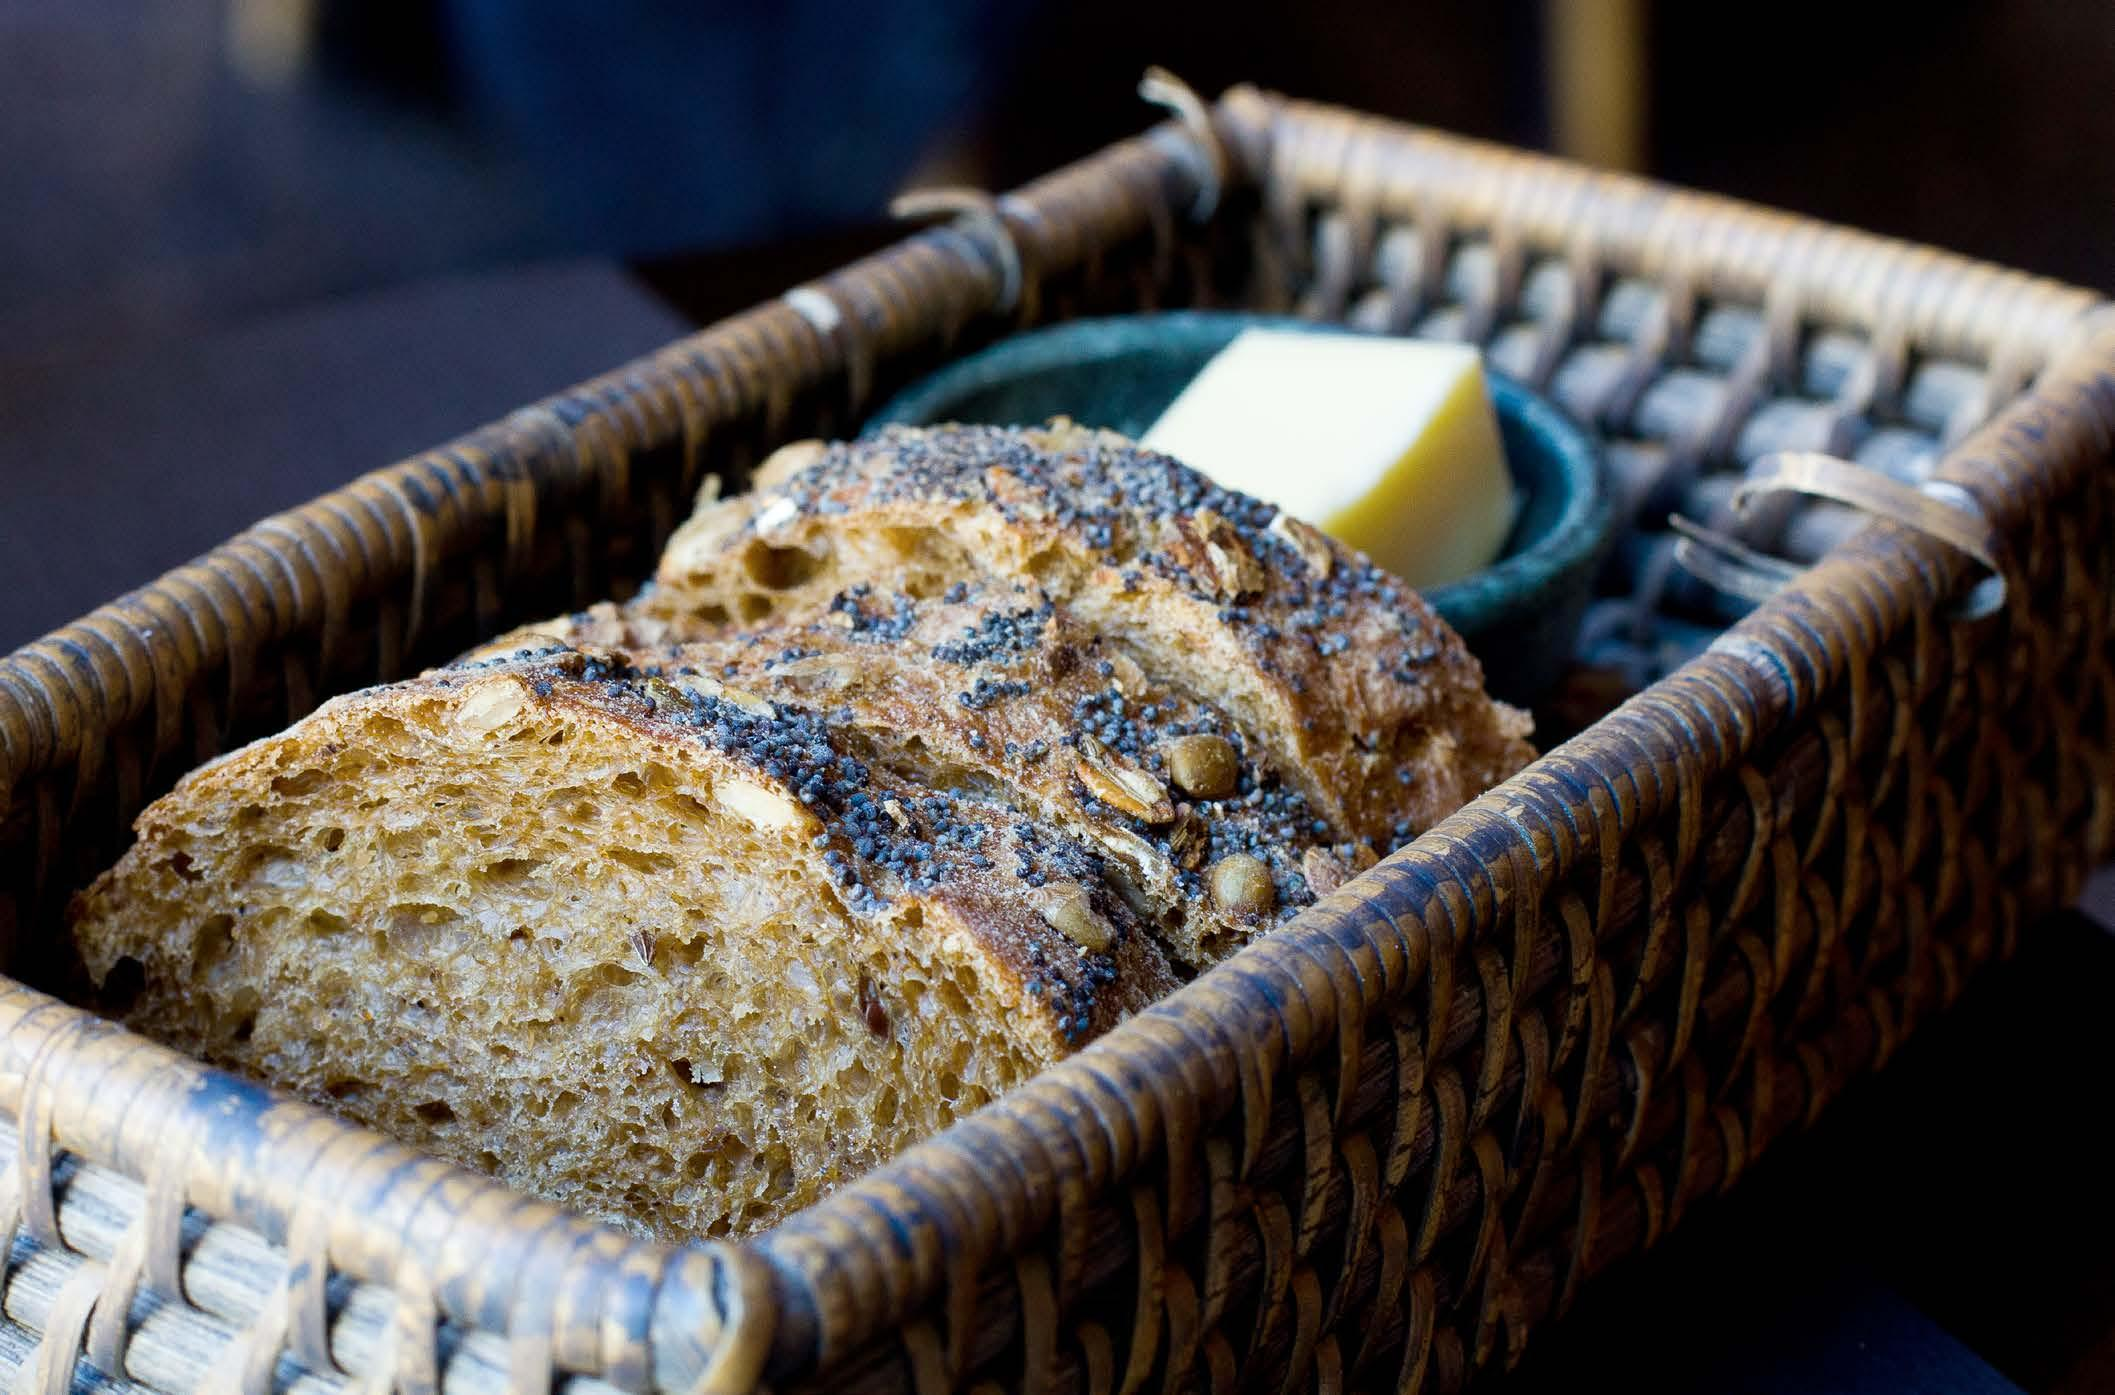
\includegraphics[scale=0.08]{depth_field_example1.jpg}
    }
    \subfigure[] {
                \label{fig:depth_field_example2}
                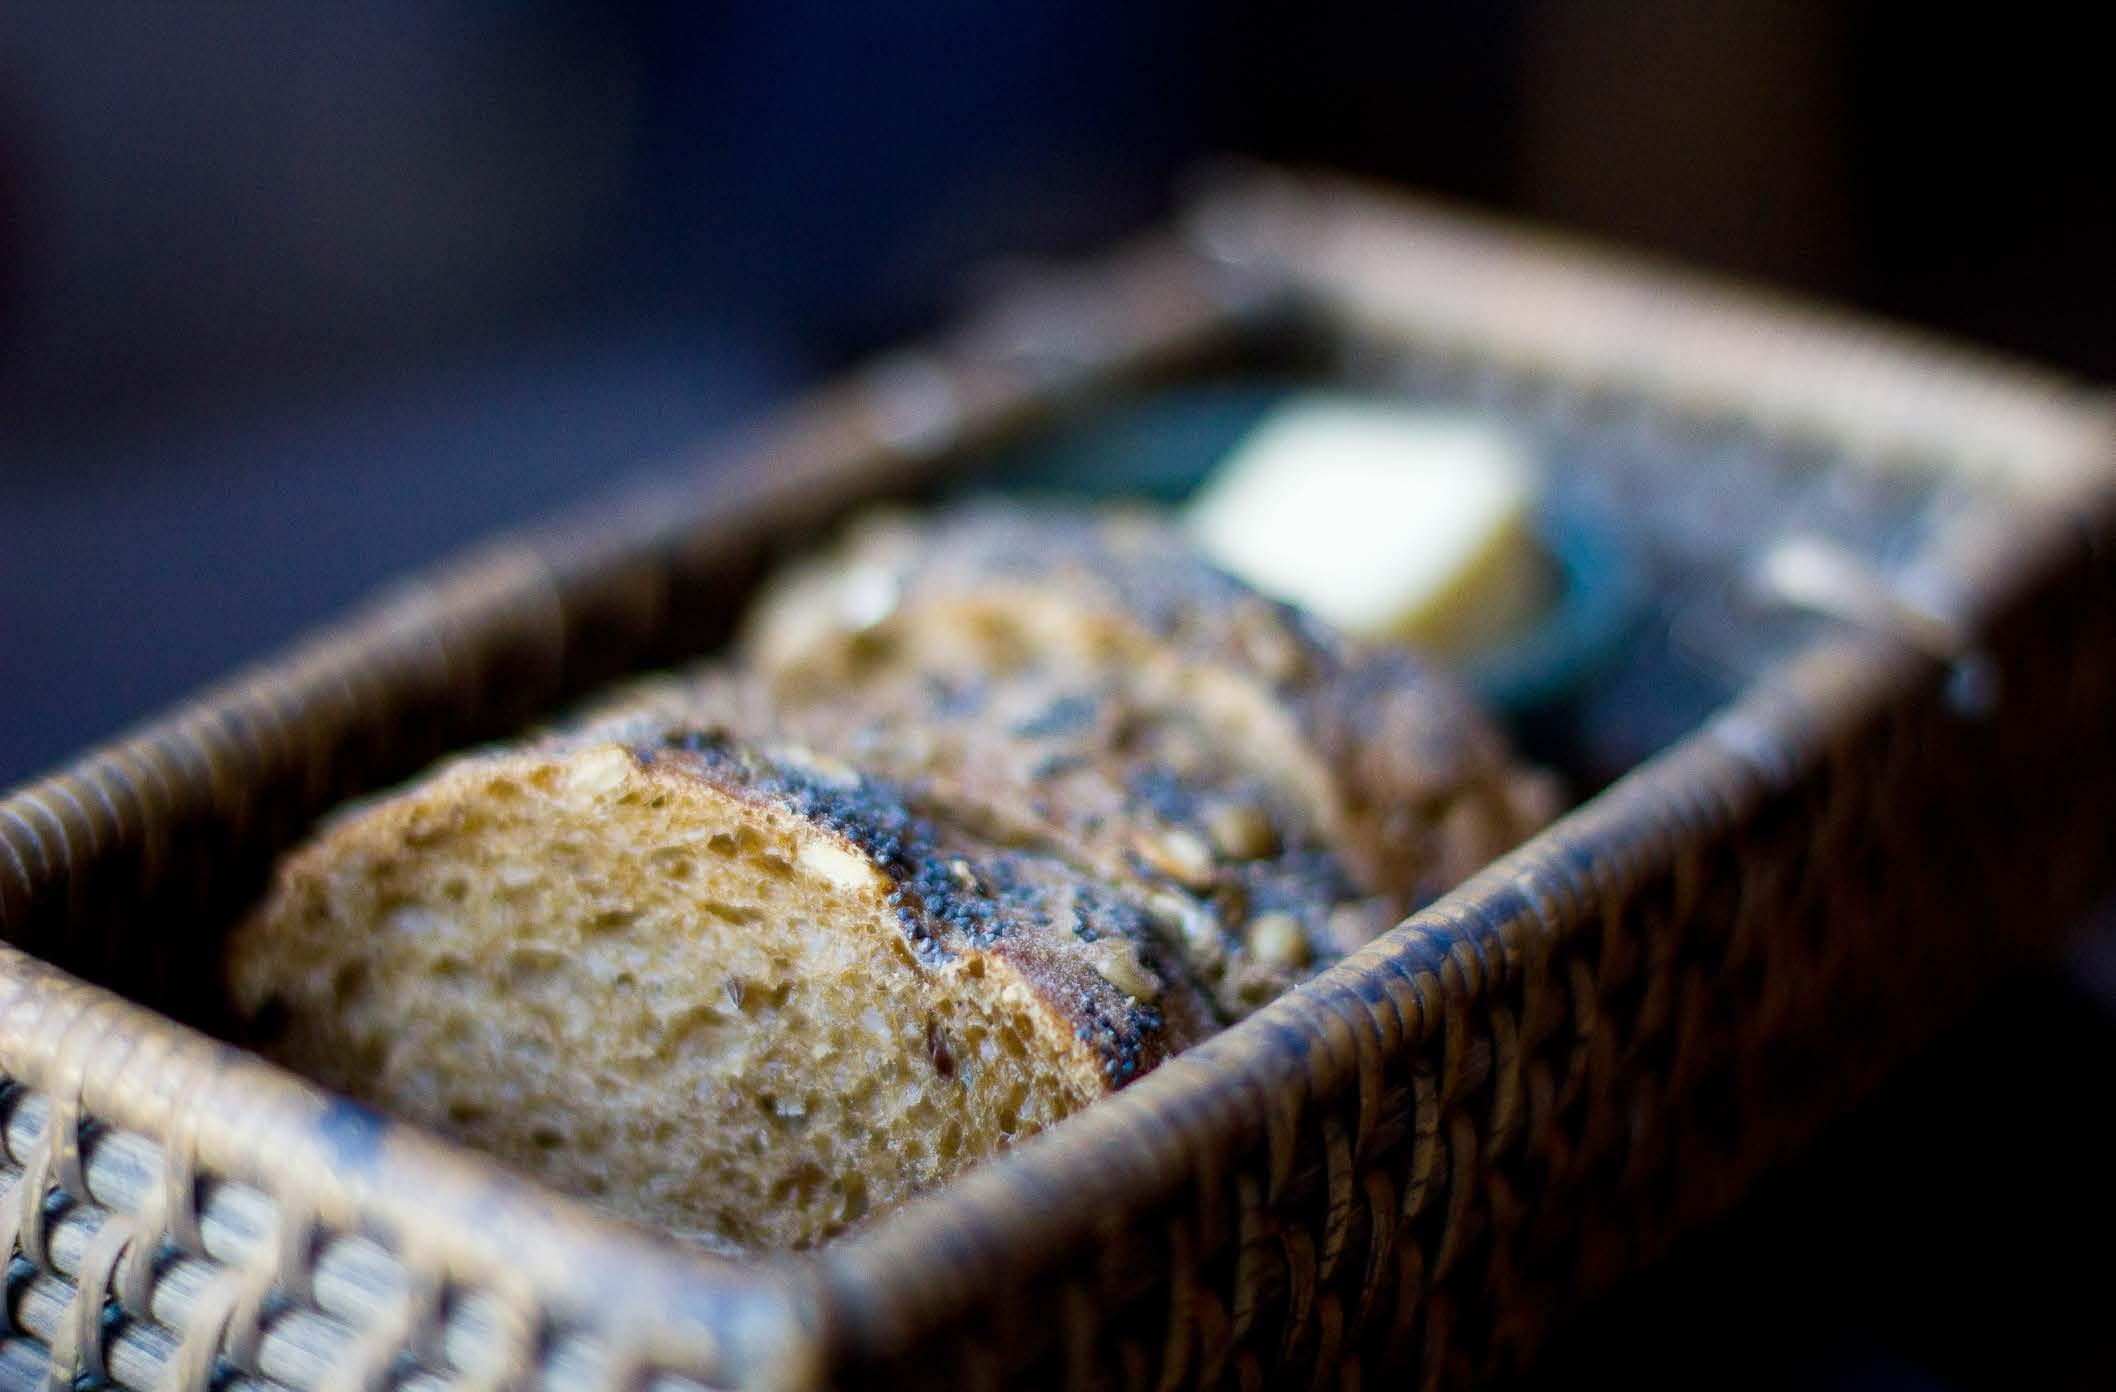
\includegraphics[scale=0.08]{depth_field_example2.jpg}
    }
  \caption{Difference between a shallow depth of field (a) and a wider depth of field (b). \cite{Kamps2012}}
  \label{fig:depth_field_example}
\end{figure}

\subsection{ISO}
\label{sub:iso}

This is the measure that defines the camera's sensor sensitivity to the light \cite{Kamps2012}. Digital cameras tend to behave better in low light conditions with higher ISO values, which means that for higher ISO values, the camera's sensor becomes more sensible to light rays.
In digital cameras and mobile devices, the sensitivity can be adjusted if necessary. However, increasing the camera's sensitivity to the light recklessly might ruin a photograph due to the fact that it will introduce some digital noise in the image, as shown in Figure \ref{fig:iso_example}. To reduce this negative effect in the image, the use of high ISO values can be compensated with fast shutter speeds and low aperture values.

\todo[inline]{Como adicionar referencia da imagem ? http://photographylife.com/what-is-iso-in-photography}

\begin{figure}[htbp]
        \centering
    \subfigure[] {
                \label{fig:iso1}
                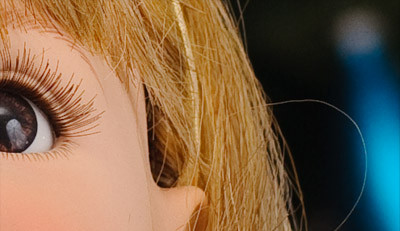
\includegraphics[scale=0.45]{iso_example1.jpg}
    }
    \subfigure[] {
                \label{fig:iso2}
                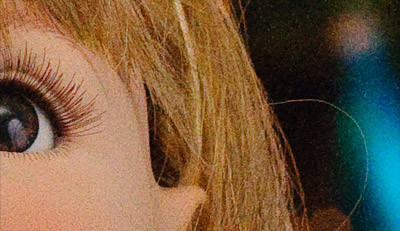
\includegraphics[scale=0.45]{iso_example2.jpg}
    }
  \caption{Difference between an image with ISO value of 200 (a) and 3200 (b).}
  \label{fig:iso_example}
\end{figure}

\subsection{White-balance}
\label{sub:white_balance}

It is a known fact that the human eye is more sensible to light variations than color variations, therefore, when we see an object reflecting light, our brain instantly interprets the color. This means that in areas of different brightness, our eyes adapt and interpret the same color, although, to the camera they are not equal.
Since camera's are not capable of simulating the human brain, that is why white-balance is used in professional photography, in order to match the captured ambience light to what our brain would read \cite{Kamps2012}. Figure \ref{fig:white_balance_example} illustrates various examples of images with different tonalities that can be corrected adjusting the white-balance.

\begin{figure}[htbp]
        \centering
    \subfigure[Too cold] {
                \label{fig:white_balance1}
                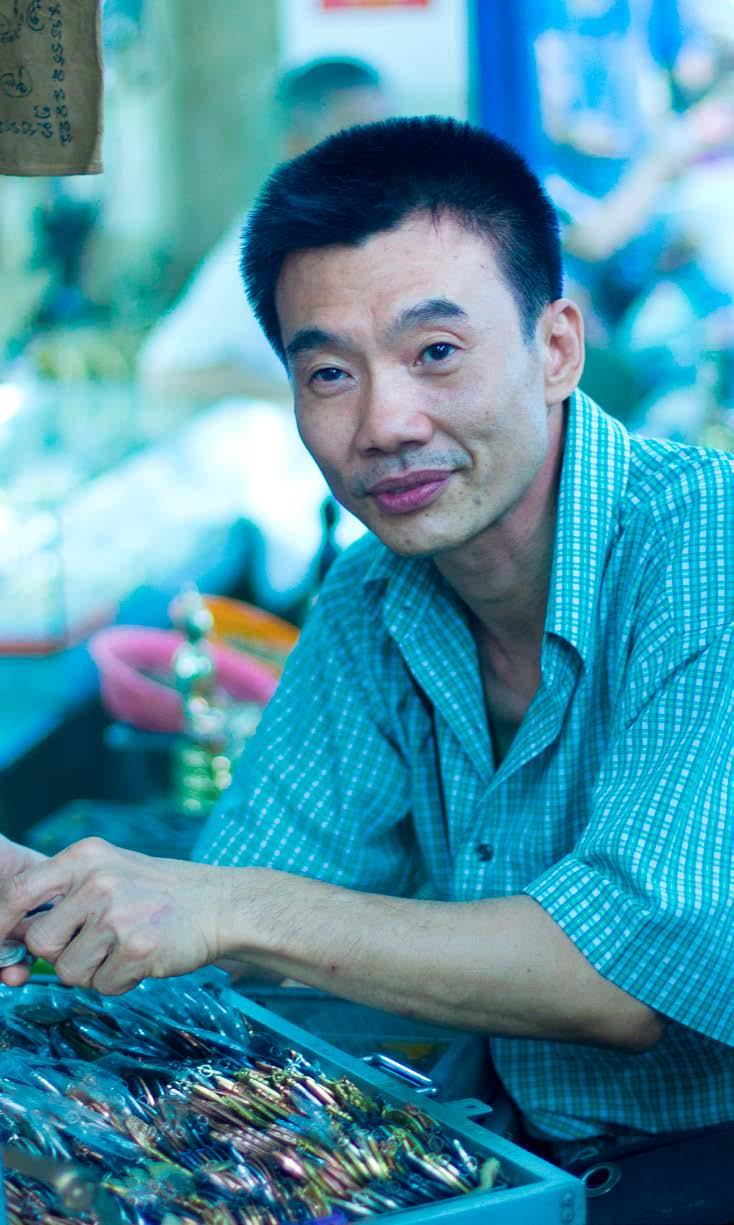
\includegraphics[scale=0.1]{white_balance1.jpg}
    }
    \subfigure[Well balanced] {
                \label{fig:white_balance2}
                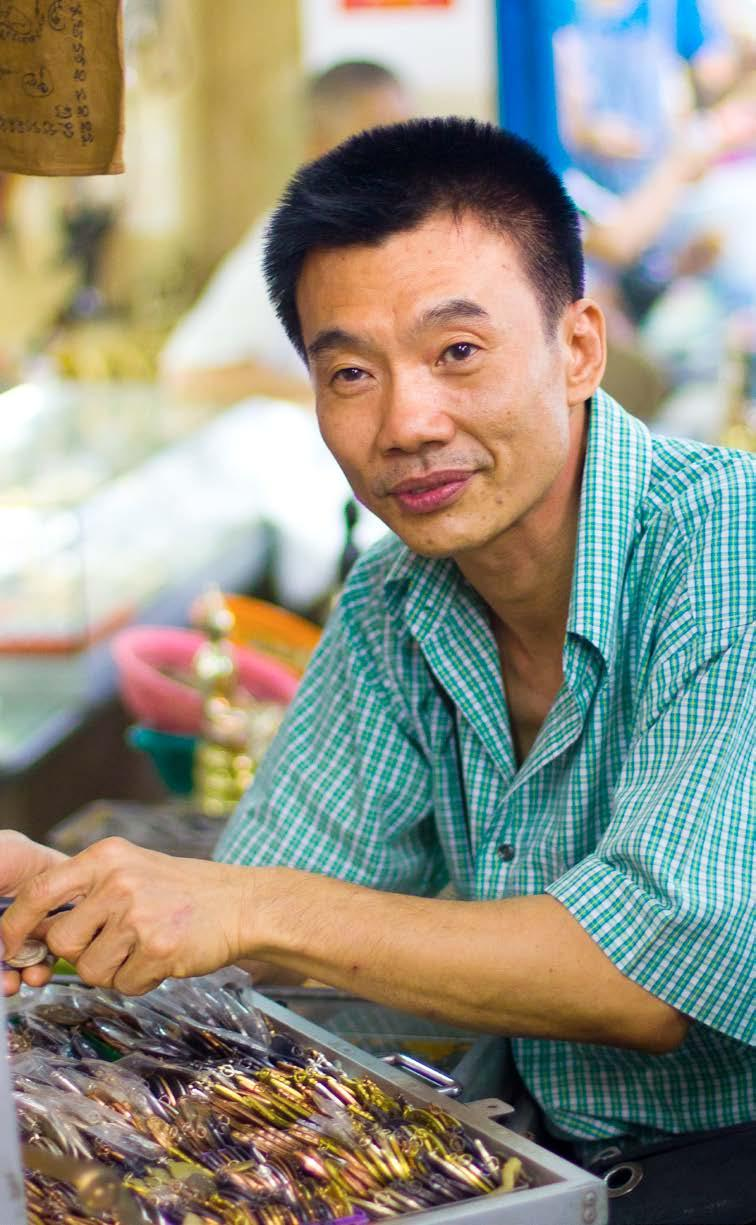
\includegraphics[scale=0.1]{white_balance2.jpg}
    }
    \subfigure[Too warm] {
                \label{fig:white_balance3}
                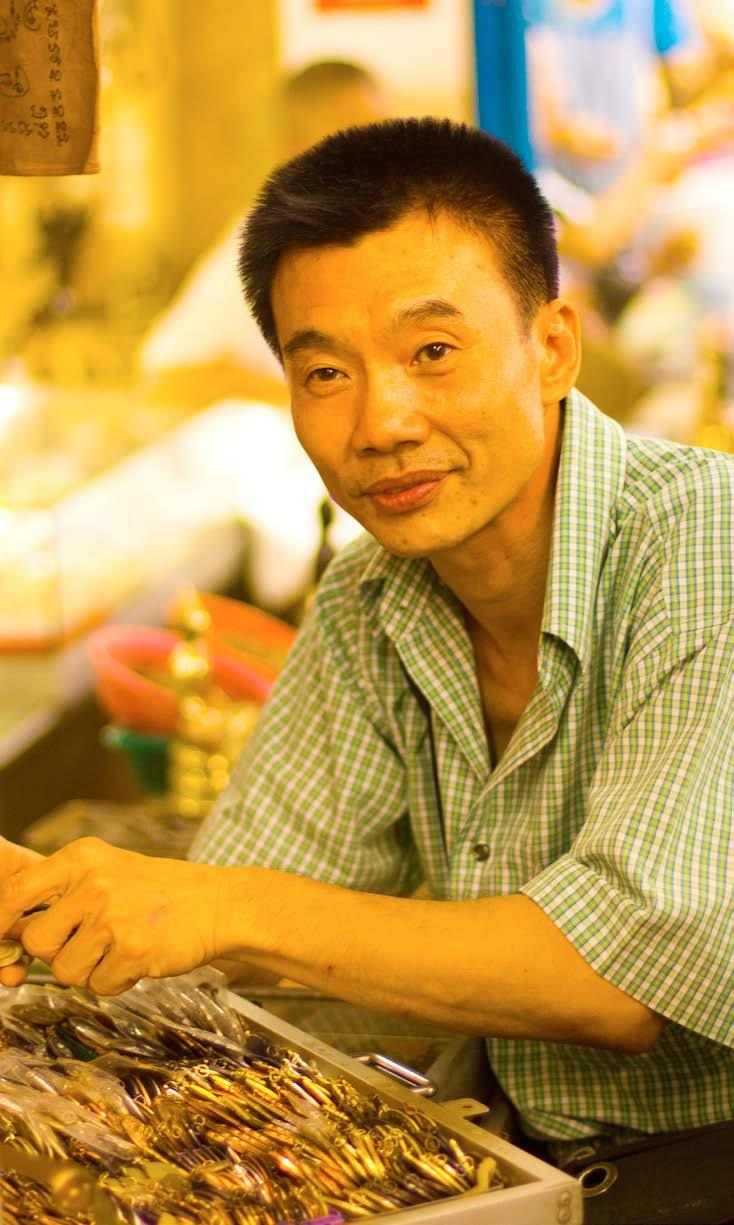
\includegraphics[scale=0.1]{white_balance3.jpg}
    }
  \caption{Three examples of white-balance applied to a photograph. \cite{Kamps2012}}
  \label{fig:white_balance_example}
\end{figure}


% ===============================================================
% =		    Processing techniques for photography				=
% ===============================================================
% # SECTION: Fundamental Concepts #



% # SUBSECTION: Processing techniques for photography #
\section{Processing techniques for photography}
\label{sub:photo_techniques}

To take advantage of the most recent capturing technology, new techniques and add-ons are being created to obtain the most pure and stunning result without any kind of editing. This techniques are achieved by exploring lenses and other concepts, such as the ones described in section \ref{sec:concepts}. This chapter will describe some of these techniques and how they can be achieved.


\subsection{Long-Exposure Photography}

Long-exposure (or time-exposure) photography exists since the popularization of photography. In the beginning, a person was obligated to stand completely immobile in front of a camera so that the final result would be as sharp as possible.
With this premise, long-exposure photography is a technique which involves taking a picture with a long shutter-speeds \cite{Kamps2012}. This way the camera sensor will record more light while the shutter is open. With such long speeds the sensor cannot record moving objects, resulting in perfectly sharp capture of stationary objects and blurring or obscuring of moving elements.
This technique is more successful under low light conditions due to the time that the sensor is exposed to light, but this can be suppressed by using special filters for the camera's lens. By taking so long to close the shutter, the sensor keeps absorbing light creating a brighter photograph producing a near daytime effect.
This technique made easier for professionals to photograph at night, and gave form to new types of photography such as light painting where a person with a light source can draw paths in the air. Being more sensitive to light, while the shutter is open, the sensor records all the paths drawn resulting in an image where the paths form a continuous line and the person or object moving the light source is obscured, as shown in Figure \ref{fig:long_exposure_example1}.

\todo[inline]{Source imagens: http://www.flickr.com/photos/awfulsara/35403447 , http://www.hongkiat.com/blog/light-painting-artworks/}

\begin{figure}[htbp]
        \centering
    \subfigure[] {
                \label{fig:long_exposure_example1}
                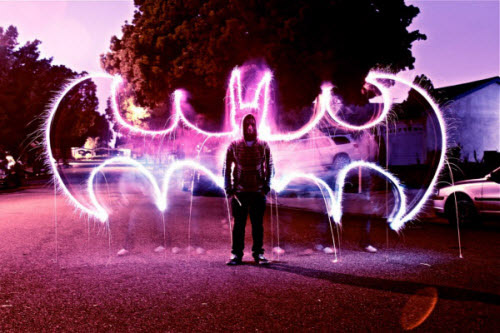
\includegraphics[scale=0.4]{long_exposure_example1.jpg}
    }
    \subfigure[] {
                \label{fig:long_exposure_example2}
                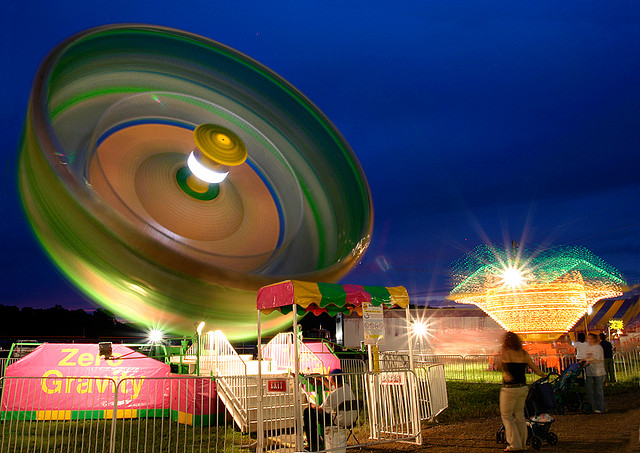
\includegraphics[scale=0.294]{long_exposure_example2.jpg}
    }
  \caption{Examples of Long-Exposure Photography. \cite{Kamps2012}}
  \label{fig:long_exposure_example}
\end{figure}

\subsection{HDR Imaging}

Although there is a big improvement in the technologies related to photography, cameras still have a problem of not being able to perceive colors the same way as the human eye. Due to that fact, depending on the exposure, different zones are represented with colors different from reality and it is possible to lose information in bright or dark zones. High Dynamic Range Imaging is based on a capture that can represent a more accurately range of intensity levels found in real scenes compensating this problem.
In photography, this technique is achieved by taking multiple Standard Dynamic Range (SDR) photographs of the same scenario with different exposure values that can vary depending on the device. After taking all the samples, the process consists in combining all the raw data of over-exposed and under-exposed areas in one image. By doing this, the image will result in a photograph with a broader tonal range, as shown in Figure \ref{fig:hdr_example}.

There have been some developments in research for architectures and algorithms that can create fast and reliable HDR images.
One of the method described in \cite{Vavilin2011} involves a three cameras, side by side, in the same optical axis that can be seen in Figure \ref{fig:hdr_camera}. Each of this cameras takes a photograph with different exposure values, taking a first picture underexposed, a second picture with the normal exposure, and a third picture overexposed. 
Since the three cameras are in different positions on the axis, the algorithm starts by aligning the three images. After the alignment, some objects in one image might be occluded in the others, so it calculates one error map for both overexposed and underexposed images in order to detect pixels that cannot be used in exposure blending because they exist in the picture with the normal exposure, but not on the other two.
To finalize, the normally exposed picture is chosen as reference. The darker pixels are combined with brighter pixels from the overexposed one. Similarly, brighter pixel are combined with darker pixels from the underexposed image, generating an HDR image that corresponds to a blending between all three samples.
\todo[inline]{Source imagens:  http://www.flickr.com/photos/wetworkphotography/7437783578/sizes/l/in/pool-1616992@N23/}
\begin{figure}[htbp]
        \centering
    \subfigure[Non HDR] {
                \label{fig:long_exposure_example1}
                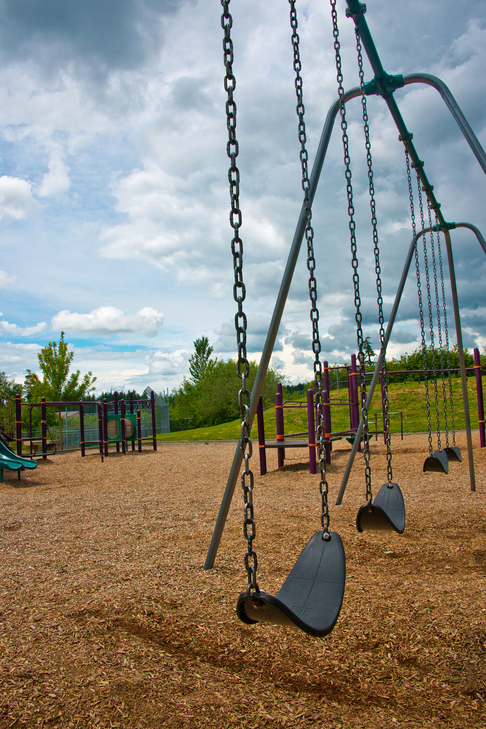
\includegraphics[scale=0.15]{hdr_example1.jpg}
    }
    \subfigure[HDR] {
                \label{fig:long_exposure_example2}
                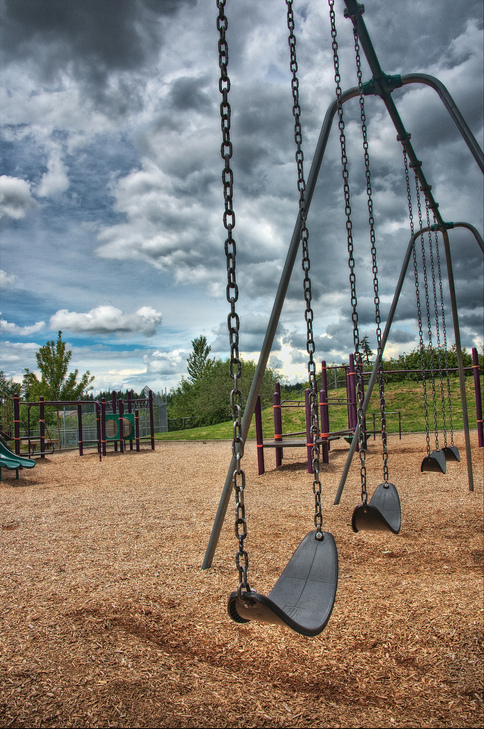
\includegraphics[scale=0.15]{hdr_example2.jpg}
    }
  \caption{Example of a picture taken with High Dynamic Range (b) versus the same picture with Standard Dynamic Range (a).}
  \label{fig:hdr_example}
\end{figure}

\begin{figure}[htbp]
	\centering
	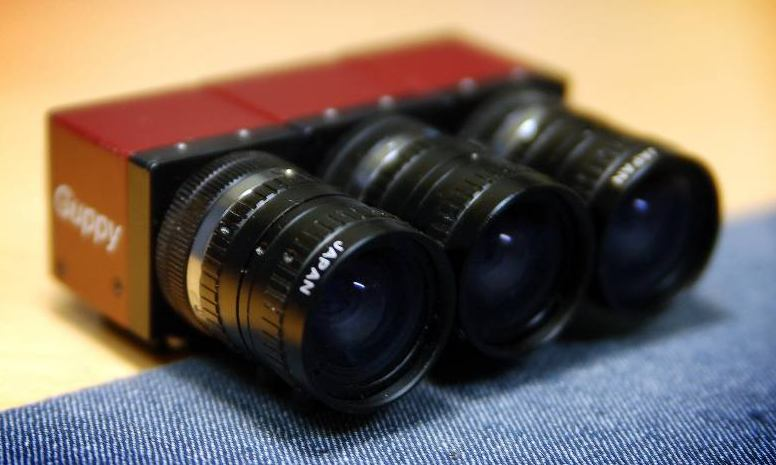
\includegraphics[scale=0.15]{hdr_camera.png}
	\caption{Image of the three cameras aligned side by side, used in \cite{Vavilin2011}.}
	\label{fig:hdr_camera}
\end{figure}

\subsection{Panoramic Photography}

Panoramic photography is a technique that creates an image with an enlarged field of view which approximates or exceeds the human eye (160º by 75º). Between specialized methods and devices, one of interest is the use of Catadioptric cameras and lenses. This cameras are based on a system of lenses and curved mirrors that allow a field of view of 360º over a single viewpoint, bypassing the need of horizontal panning as it occurs with other methods. Since it uses mirrors and lenses, the light rays bent preventing any kind of distortion or chromatic aberration. Without the need of computation, another advantage is the use of this cameras for video shooting of 360º panoramas. 
There are on the market some add-on lenses for mobiles devices that make this technique possible, such as GoPano micro (Figure \ref{fig:gopano}).

There are also methods to generate panoramas by stitching multiple horizontal images through software. \citeauthor{Szeliski} describes \cite{Szeliski}, a method to create full view panoramic mosaics. 
Unlike many other stitching methods, this algorithm does not need a set of pure horizontal images. Instead, as long as there is no strong motion between sampled images, there are no constraints on how images are taken. This makes photographs taken by hand-held devices without a tripod a reliable source for creating panoramas. According to \citeauthor{Szeliski}, the center point of the sampled images can be described in 3D by a set of matrices which correspond to the image plane translation, the focal length scaling and a 3D rotation matrix. After estimating the mean focal length of the images and rotation matrix, they can stitch the images in a 3D dimensional space.
Since it is made by stitching multiple images, the final product presents distortions at the north pole. This is because of a necessary warp to cylindrical or spherical coordinates (Figure \ref{fig:panoramic_image}) to have a full view of the panorama without using a specialized viewer.

\begin{figure}[htbp]
        \centering
    \subfigure[] {
                \label{fig:gopano}
                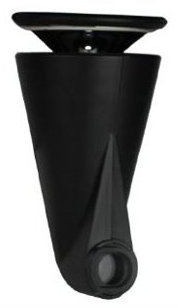
\includegraphics[scale=0.3]{gopano.jpg}
    }
    \subfigure[] {
                \label{fig:long_exposure_example2}
                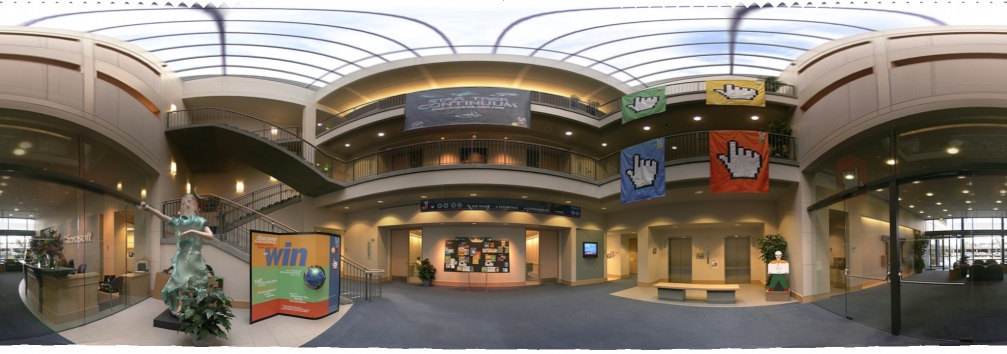
\includegraphics[scale=0.45]{panorama_example.jpg}
    }
  \caption{Image of attachable lens for iPhone, GoPano micro (a), and panorama made by the algorithm described at \cite{Szeliski} with distortion at the north pole.}
  \label{fig:panoramic_image}
\end{figure}



% # SUBSECTION: Image capturing and processing apps #
\section{Image Capturing and Processing}
\label{sub:capturing_processing}

Since the first attempts to capture a scenery by Thomas Wedgwood, to its popularization in the XIX century, the world of photography has suffered improvements, that still shock many professionals in the business. Since the upgrade of analog cameras to the digital world, the use of negatives and dark rooms to new techniques like tilt-shift and HDR, the current market has been increasingly overwhelmed by mobile devices and their ability to easily dethrone today’s digital cameras. Proof of this fact is the wide range of applications related to photography presented in mobile devices application stores like Google Play and App Store. Some with a more professional objective than others, throughout this chapter, it will be discussed some of those applications for image capturing and processing. Along with these applications, some investigation that has been done in this field, will also be discussed.

\subsection{Image Capturing}

\subsubsection{Android and iOS Native Applications}

By default, the newest mobile operating systems, already have an incorporated application to take photos. For example, on iOS, the default application is rather simple. It has very few customization options for a user who pretends to capture scenes to a more professional level, although it is possible to record videos and choose between full screen photos or photos with a squared format, using one of the two cameras available, with or without flash. Besides these, iOS native application offers a shortcut to access the device’s gallery.

On the other hand, android’s native application is a flexible alternative, in such a way that offers access to functionalities, allowing the user to take the advantage of how she can capture the scenery, in the likeness of today’s digital cameras.
Some of these options include messing around with ISO and exposure values, white-balancing, contrasts, and choose the resolution of the final product. It allows the user to choose the correct capture mode for the moment, e.g. sports mode, indoor, portrait, etc.
Android’s application has a nice tweak, it is possible to add metadata tags to the image which may include GPS location a rename the file based on that location. It also becomes user friendly, when it displays a grid on the screen, helping the user to center the object that is being photographed. Despite all the options, one of the main features is the anti-shake system that applies corrections on the image to compensate user’s movements.

\subsubsection{Instagram (iOS)}

With already a notorious percentage of popularity and very centered in social networking, Instagram is an application that offers the main features of a native application. Some of these features include the possibility of taking a photograph or record a video and choose between between the front and rear camera, if they both exist on the device. With direct access to the device’s gallery in both modes, the shooting mode, in similarity with Android’s default, shows a grid in the display, and control options for flash.
The presence of menu bars at the top and bottom of the screen reduces the space available to preview the shoot and maintains a squared shape for both the preview and the shoot taken, as shown in Figure X.


\subsubsection{Photoshop Express (iOS)}

Tool developed by Adobe that has a shooting mode with some extra features in comparison with the native application. Some of these extra features are the timer option and a preview of the image taken.
Between these two, the preview is an interesting option to be used in a more professional context allowing the user to decide if it is an usable photo before saving it in the gallery.
Although in most of the available applications, the zoom feature is already a given, in Photoshop Express it can be controlled by an horizontal slider. This fact that is an horizontal slider always visible, comes in handy to the user because it is understand how to make zoom comparatively to the default applications. 
In those default applications, the user can perform a zoom by pinching the screen which may not be intuitive. This way, the horizontal slider may be a good alternative for a more intuitive interface.

\subsubsection{Photosynth (iOS)}

In resemblance to Instagram, Photosynth was developed by Microsoft, with the objective of creating a social network centered in sharing panoramic photos. The social features will be ignored since they are not the main topic of this thesis.
Regarding the image capturing abilities, this application allows the user to create a software generated panoramic image. For capturing, the device displays a 3-dimensional spherical space that rotates with the user’s movement. As soon as the capture starts, Photosynth automatically captures the initial scene and all the adjacent scenes while the user is rotating. After finishing the capture, this application identifies specific features in one photograph and matches with other photographs features and by analyzing the position of matching features within each photograph thus identifying which photographs belong on which side of others and identifying images of the same area. 
To visualize the panoramic image, the stitched images are displayed in a 3-dimensional spherical space similar to the one presented on the capture display, with the particularity that the user must scroll to see the final result. Outside the application, previewing the image in the gallery, it presents some deformations that were required in order to represent it in the 3 dimensional dome inside Photosynth. 


\subsubsection{Camera FV5 (Android)}

Camera FV5 is by far, one of the most complete applications for photography in the Play Store market. Although it has a screen with lots of options and information, it is what most resembles to a digital camera display. It offers full control over exposure, ISO and white-balance. Exposure can be manually selected by the user or, alternatively, she can choose between modes that automatically determine exposure values based specific regions of the image displayed in viewfinder. 
Multiple focusing modes are available, that allow macros, setting the focus to infinity or taping the display and select the object to focus.
More related to camera utilities, various flash modes are available, including a flashing mode that fixes red eyes on photos, shooting utilities which include a shooting timer, image stabilization and burst mode.
For a more inexperienced user, default programs with pre-defined exposure options can be used.
The most interesting trait are the indicators in the viewfinder that display values of exposure time, aperture, ISO, battery remaining and how many photos are in buffer.
The fact that it allows all photographic parameters to be controlled, it makes possible the creation of photos with photography techniques like long-exposure, although, due to hardware limitations, this technique is all emulated by software and not with the hardware.

\subsubsection{SketchCam}

SketchCam appears as an investigation project that uses a different approach towards mobile devices as photography. With a touch screen, it enables children to capture images by sketching the area of interest on the display. 
Using this different approach, it allows the user to become more selective towards the scenario in front of her, and creative, in a way that the user may be able to create different frames for the picture that is being taken.  After selecting the point of interest in the view display, it creates an object that can be used for future collages. This may help teaching the basic concepts of composition and photo editing by using a different display. 


\subsubsection{Frankencamera}

Although there are many mobile devices with capabilities to take photos, most of them don’t take full advantage of the imaging hardware and offer a highly simplified API. The programmer can’t control the camera’s exposure time or retrieval of raw sensor data. Based on this problems, Frankencamera is an open-source architecture with a custom-built camera based on Linux and gives full control of the hardware to the programmer through C++ language. This architecture consists in an application processor, a set of photographic devices such as flashes and lenses, and one or more image sensors, each with a specialized image processor, forming a tightly coupled pipeline to coordinate all elements. All sensors, devices and parameters that describe the capture and post-processing of a single output image, can be programmed through its API allowing a mechanism to precisely manipulate the hardware state over time.
Being a custom made platform, brings some advantages towards closed platforms. One of these advantages is the ability to take long-exposure photos without a tripod. Using an embedded gyroscope, the camera will stream full-resolution raw frames that will be stored, only if their gyroscope tags indicate a low motion when the frame was taken. 
Another useful application is the creation of panoramic photos with extended dynamic range. In most devices, the user has to take various individual photographs and stitch them together on a computer, but with this system, it is possible to individually set the exposure time of each shot creating a panorama with extended dynamic range and previewing the result instantly.

\subsubsection{Discussion}

All commercial applications and research projects share the most basic features that should come embedded in any system takes photos. These features include access to a gallery, control over flash, control which camera to use, an auxiliary grid and control over zoom.
In order to dethrone digital cameras, stock applications such as the ones that come by default with Android and iOS, started that process of mass dissemination of a portable, simple and completely capable option to take casual photos. 
Android applications, comparatively to iOS, offer more control over the device’s hardware, such as shooting mode, resolution and image quality, aperture and ISO values. Allowing almost full control of the hardware to the user, is a very important feature that must taken in consideration when developing an application to take photos. Given this fact, Android becomes a more reliable platform for users that pretend to use their mobile device for something more than casual photos.
With some interesting features, Camera FV5  is one of those applications for amateur photographers that presents very similar interface to a digital camera with a possibility of adjust all photographic parameters and introduces the emulation of some photography techniques.
Interesting features that should be noted on Photosynth, is the way the application handles the creation and preview of panoramas. The existence of a spherical 3-dimensional that takes multiple photos and detects differences according to the previously taken, is an automated process that can be easily learned by every user.
In the research field, SketchCam and FrankenCamera can go beyond what is available on regular systems. Although designed for kids, Sketchcam presents a system with a very different way to interact with the user in how she takes a photo. Selecting the point of interest by sketching a continuous path and giving form to different shapes of frames in a display with a live video feed, can be handy when a user only wants to emphasize a region or object in the viewfinder.
Frankencamera is allowing computational photography to take a step further. It is the perfect of what is possible by taking full advantage of a device capabilities. It allows to take long-exposure photos using the available gyroscope proving that better photos can be taken using multiple sensors available.

%------------------------------------------------------------------------------------------------------------------
%------------------------------------------------------------------------------------------------------------------
%------------------------------------------------------------------------------------------------------------------

% # SECTION: Avaliação de Fotografia #
\section{Image Evaluation}
\label{sec:photo_eval}
To understand aesthetic problems, \citeauthor{Hoenig2005} in \cite{Hoenig2005}, described and formalized a set of theorems and components that could provide a measurable basis for aesthetics.
According to the author, in 1933, George David Birkhoff came up with a formula that encapsulated his insights into a aesthetic value, described by $ M = Order/Complexity $. This represents the reward one gets, by experiencing orderliness while putting effort in focusing details, giving higher aesthetic value to beauty over complexity. Birkhoff's concept sparked interest of computer scientists in aesthetics, creating the term computational aesthetics. This therm is described as a set of computational methods that can make applicable aesthetic decisions in a similar fashion as humans can.

%A professional photographer might have a good equipment, the perfect light and a good control over exposure, but one key feature is the composition of the picture. Many of the rules of composition used by photographer have been copied from classical painters.
%Photographers have the challenger of taking an interesting photography, and a good composition encourages the viewers eyes to roam around the image and capture hers attention.
%There is no recipe for a good composition, and for that reason a photographer must have in consideration of how an image is read by the majority of population. The inherent tendency to sweep an image from left to right, and from top to bottom, with the knowledge of how the human eye reacts to color, luminosity, directing lines are facts that are taken in account when shooting and when evaluating an image. This section contains two subsections where this concepts will be explained in the first one and some approximations of their use for evaluation will be introduced on the later.

% # SUBSECTION: Regras de Composição #
\subsection{Composition Rules}
\label{sub:photo_rules}

To obtain aesthetic results, photographers follow certain rules of composition that are the result of centuries of artistic development. These rules are now considered as rules of thumb, and proven to be pleasing to the eye.
There is no recipe for a good composition, and for that reason, a photographer must have in consideration of how an image is read by the majority of population. The inherent tendency to sweep an image from left to right, and from top to bottom, with the knowledge of how the human eye reacts to color, luminosity and  lines, are facts that need to be taken into account when shooting. This section describes of the rules that captures the viewers attention and can be used in computational aesthetics.

\subsubsection{Color Balance}
\label{subsub:color_balance}

Although a good photography is dependent on the subject that is being captured, color has a major impact in creating a certain mood and empathy with the viewer. 
%In digital photography what is captured is the transmitted light and not the reflected light, the primary transmitted colors are composed by red, green and blue (RGB), and consequent secondary colors obtained by merging this three components. 

It is rare for a color to be isolated in a photo shoot, and depending on the color palette, a different relation between them will be established. These relations can create similar or different emotions that can be explored in a composition \cite{Santos}.
A relation created by two complementary colors gives a sensation of balance, but if both colors have different luminosity values, the less luminous color must be present in a greater amount comparing to its complement (Figure \ref{fig:color_balance_image}).
To evoke a mood and arouse emotions, each color has its own meaning that can be interpreted in different ways by different cultures. For the western civilization, yellow symbolizes cheerfulness, joy and optimism, but for the eastern civilization, it is related to the imperial kingdom and symbolizes something sacred. On the other hand, in the Egypt, is a color for mourning.

\begin{figure}[htbp]
    \centering
	\label{fig:color_balance_example}
    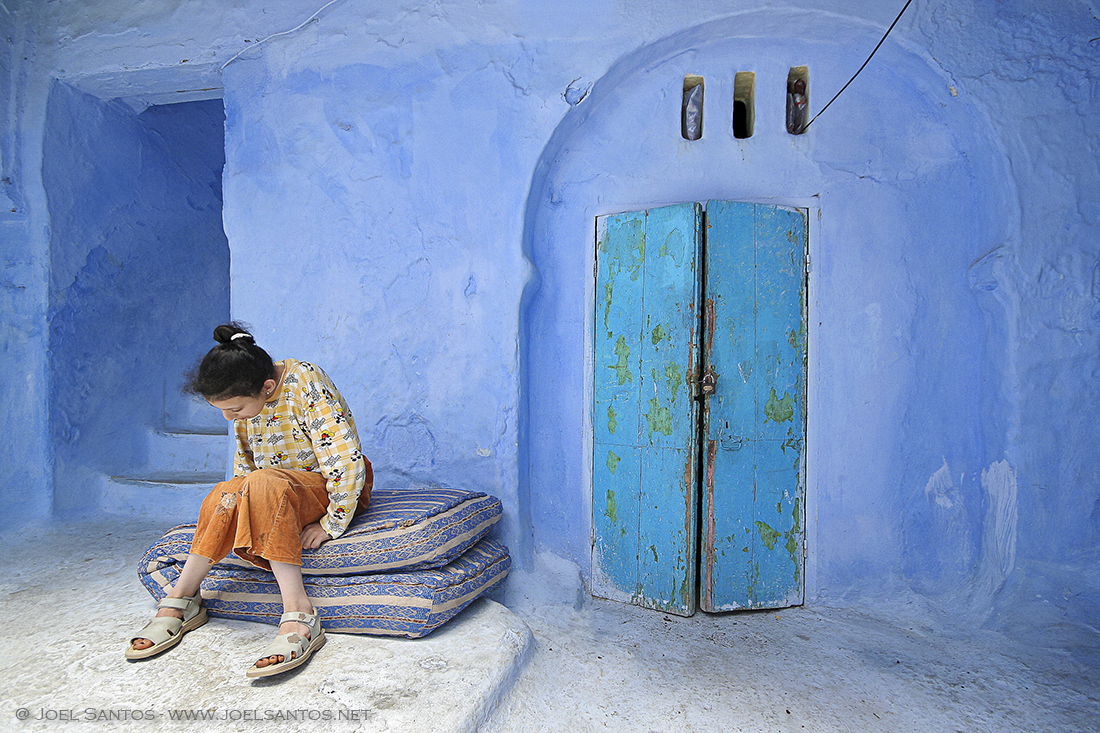
\includegraphics[scale=0.3]{color_balance_example.jpg}
  \caption{Image of two complementary colors balanced in a frame. \cite{Santos}}
  \label{fig:color_balance_image}
\end{figure}

\subsubsection{Rule of the Golden Section and Golden Spiral}
\label{subsub:golden_section}

Rules used by many photographers, artists, architects, and considered to obtain very appealing and aesthetic results. The golden section rule is based on the golden average. This value can be achieved from a division between two consecutive numbers in a Fibonacci sequence. For example, defining the sequence [8,13,21] as a subsequence of the original Fibonacci, dividing 13 by 8, and 21 by 13 will result in a ratio, that in the limit, will be equal to the golden number (i.e. $\approx 1.6180339$). This golden number is what defines a golden section \cite{Santos}. 

This section, which is believed to be aesthetically pleasing, consists of a group of rectangles in which the ratio of the longer side to the shorter is equal to the golden ratio. It is possible to draw a logarithmic spiral whose growth factor is equal to this ratio, called the golden spiral, which converges to the smallest rectangle in the section. From this point onward, the convergence point will be treated as \emph{power point}. 

With this concept, it is possible to create a grid formed by the intersection of vertical and horizontal lines that pass through four specific points. The points correspond to \emph{power points} obtained by converging a golden spiral from each vertex of the golden section (Figure X). This grid will result in a guideline with reference lines and imaginary points that indicate where the main subject of the scene should be located, usable in portrait and landscape mode.

\subsubsection{Rule of Thirds}
\label{subsub:rule_thirds}

The rule of thirds is based on the golden section. While this last one results in a guideline where the \emph{power points} respect the conversion point of a golden spiral, the rule of thirds consists in dividing the rectangle in nine equal parts. The scene is divided in thirds both horizontally and vertically with power points at the intersections \cite{Santos}.
Being a derivation of the golden section, the fundamental concept of where the object should be, remains the same. The main subject should be positioned in one of the \emph{power points} and along the the lines, as shown in Figure \ref{fig:rule_of_thirds_image}.

\begin{figure}[htbp]
    \centering
	\label{fig:rule_of_thirds_example}
    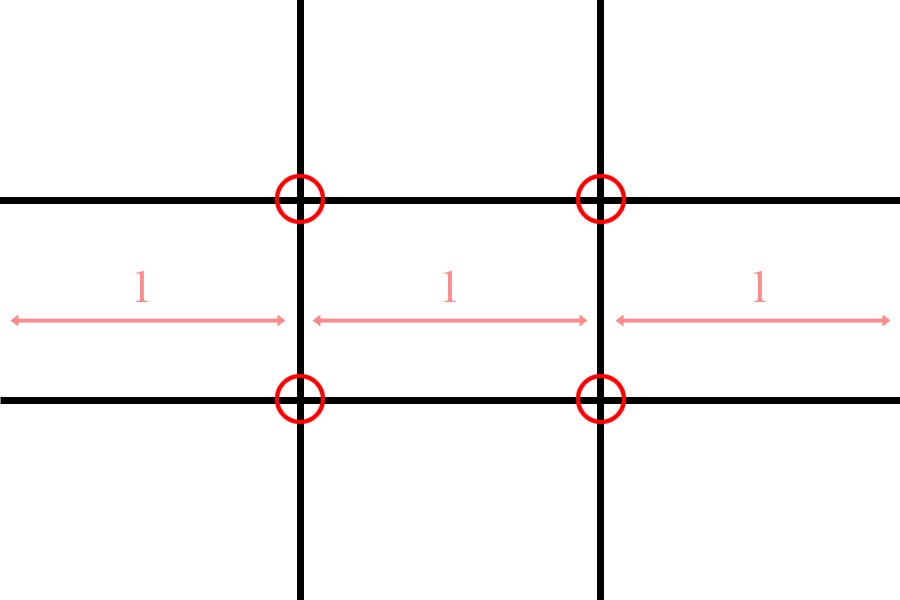
\includegraphics[scale=0.2]{rule_of_thirds.jpg}
	\caption{Guidelines of the rule of thirds with nine equal rectangles and respective \emph{power points} circled in red.}
	\label{fig:rule_of_thirds_image}
\end{figure}

\subsubsection{Golden Triangles Rule}
\label{subsub:rule_triangles}

The golden triangles rule uses a group of triangles that follow the proportions described by the golden section. Using a golden section, we draw a diagonal line between two corners of the rectangle and connect a perpendicular line to each of the remaining corners. In some cases, this can be simplified to only one perpendicular, having only one power point in the intersection with the diagonal line and a suggestive region in the frame to place the elements \cite{Santos}.

\begin{figure}[htbp]
    \centering
	\label{fig:golden_triangle_example}
    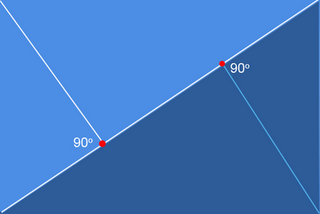
\includegraphics[scale=0.5]{golden_triangle.png}
	\caption{Guidelines obtained by the golden triangles rule.}
	\label{fig:golden_triangle_image}
\end{figure}

\subsubsection{Usage of leading lines}
\label{subsub:leading_lines}

Lines can be used implicitly by creating an imaginary line between two subjects in a picture, or explicitly, like the edges of a building. These lines can be formed of just about anything, and have the purpose of leading the viewer to a specific area enhancing the subject being photographed \cite{Kamps2012} (Figure \ref{fig:leading_lines_image}). These lines can be vertical, horizontal, diagonal or curved.

Since humans have binocular vision, unconsciously, horizontal lines are easier to interpret and give a sensation of stability and safety. Vertical lines can delimit the begin and the end of a scene, and work as an enforcement for horizontal lines.
Free of interpretations, diagonal lines are responsible for creating perspective in a photo. If the photo does not have a specific subject to photograph, diagonals can direct a viewer to outside of the frame, but on the other hand, the viewer eyes can be imprisoned by using straight angles. 
Curved lines can have an number of angles, and for that reason, they can give a sensation of movement. Although, depending on the subject and depth of field, the same curves, might have different results.

\todo[inline]{source: http://digital-photography-school.com/how-to-use-leading-lines-for-better-compositions}

\begin{figure}[htbp]
        \centering
    \subfigure[] {
                \label{fig:leading_lines1}
                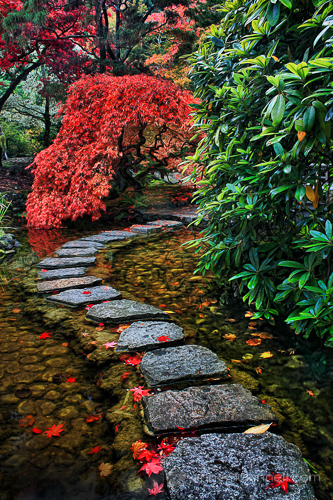
\includegraphics[scale=0.4]{leading_lines1.jpg}
    }
    \subfigure[] {
                \label{fig:leading_lines2}
                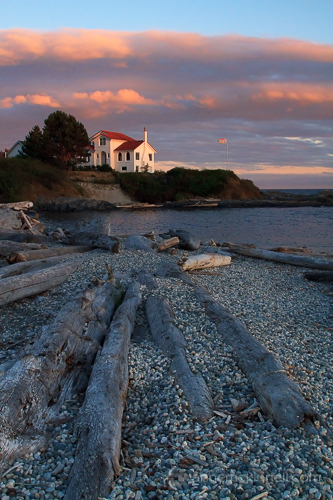
\includegraphics[scale=0.4]{leading_lines2.jpg}
    }
  \caption{Examples of a curved line (a) that redirects the viewer's eye to the maple tree, and vertical lines (b) redirect the subject in the photo.}
  \label{fig:leading_lines_image}
\end{figure}

\subsubsection{Balance of elements}
\label{subsub:balance_elements}

Unconsciously, the human mind evaluates a photo and look if there exists any balance or unbalance between the elements \cite{Santos}.
To judge the balance between the elements of a composition, we must imagine a frame divided by two and a scale that will measure the weight of the left side with the right side.
When the scale is perfectly balanced which is very common in symmetrical images, it means that both sides have the same weight visually, creating what is called static balance.
In dynamic balance, it is possible to create a balance in the image between with two imbalanced sides. This can be achieved if one of the sides has a larger element but the remaining side has a smaller but brighter object.
The scale doesn’t have to be perfectly balanced and a strong composition can be created with unbalanced sceneries. This way, the viewers attention will lie over the same side, empowering the subject in the frame.


\subsection{Practical Application of Aesthetic Evaluation Systems}
\label{subsub:eval_applications}

\todo[inline]{Falar de \cite{Liu2010}, \cite{Liu2010a}, \cite{Lok2004}?}

As referred in \ref{sec:photo_eval}, computational aesthetics can be described by aesthetic decisions made by computational methods. Increasing aesthetic awareness, researches developed systems and algorithms that extract and evaluate features of an image based  in the rules described at \ref{sub:photo_rules}.

Defining aesthetics as a \"concern with beauty and art and understanding of beautiful thing\", \citeauthor{Datta} described in \cite{Datta}, a system capable of extracting visual properties of images and automatically tell the difference between aesthetically pleasing and displeasing images. 
Based on a data extracted from an online photo sharing community, a set of images and aesthetic ratings given by the community, were used in to train a classifier.

In photography and color psychology, color tone and saturation have important roles, and for that the images were converted from \emph{RGB} to \emph{HSV} color space, producing two-dimensional matrices for each of the components. There were extracted a total of 56 candidate features related to image properties, e.g. exposure, hue, saturation, size and aspect ratio, and composition, e.g. rule of thirds, use of texture and shape convexity.
From all the candidate features, it was selected a total of 15 visual features that established a significant correlation between the visual properties of photographic images and their aesthetics ratings given by the community. The selected features would later be used by the classifier to attribute a rating to an image.
This system was later to build an interface that would determine the aesthetic value of an image submitted by a user \cite{Datta2010}.

Similar systems have been implemented. In \cite{Yeh}, \citeauthor{Yeh} described mutable ranking system. This system listed 1000 ranked photographs ordered from the highest rank to the lowest. The score of each photograph was considered as a linear combination of each feature and its corresponding optimal weighting factor that is found after the extraction of features. However, since the optimal weights might not combine with the users preferences, it enables them to combine personal taste with a trained model, and rearrange the ordered list of ranked photographs.
The weighting adjustments can be feature-based where the user can personally select the weight of each feature, or an example-based approach, where she selected a photograph they like and have the system update the weighting based on the example chosen.
The features chosen to extract, are quite similar to the ones used in \cite{Datta}, but introduce an interesting composition rule. They extract the subject region and assess the simplicity of a photograph by the color distribution of the remaining region that corresponds to the background.


